%%%%%%%%%%%%%%%%%%%%%%%%%%%%%%%%%%%%%%%%%
% Thin Sectioned Essay
% LaTeX Template
% Version 1.0 (3/8/13)
%
% This template has been downloaded from:
% http://www.LaTeXTemplates.com
%
% Original Author:
% Nicolas Diaz (nsdiaz@uc.cl) with extensive modifications by:
% Vel (vel@latextemplates.com)
%
% License:
% CC BY-NC-SA 3.0 (http://creativecommons.org/licenses/by-nc-sa/3.0/)
%
%%%%%%%%%%%%%%%%%%%%%%%%%%%%%%%%%%%%%%%%%

%----------------------------------------------------------------------------------------
%	PACKAGES AND OTHER DOCUMENT CONFIGURATIONS
%----------------------------------------------------------------------------------------

\documentclass[a4paper, 11pt]{article}

\usepackage[protrusion=true,expansion=true]{microtype}
\usepackage{graphicx}

\usepackage{mathpazo} % Use the Palatino font
\linespread{1.05} % Change line spacing here, Palatino benefits from a slight increase by default

\makeatletter

\renewcommand{\maketitle}{
	\begin{flushright} % Right align
		{\LARGE\@title} % Increase the font size of the title
		
		\vspace{30pt} % Some vertical space between the title and author name
		
		{\large\@author}
		\\\@date
		
		\vspace{20pt} % Some vertical space between the author block and abstract
	\end{flushright}
}

%----------------------------------------------------------------------------------------
%	TITLE
%----------------------------------------------------------------------------------------

\title{\textbf{Formatted Images from Matplotlib}}

\author{\textsc{Derek Kozel}}

\date{\today}

%----------------------------------------------------------------------------------------

\begin{document}
	
	\maketitle
	
	\section*{Introduction}
	
	This document shows the integration of a plot created using Matplotlib in such a way that the text formatting is consistent with the rest of the document.
	\newline\newline
	\noindent Adding the following:
		
	\begin{verbatim}
		This text area is \the\textwidth wide.
	\end{verbatim}
	
	\noindent Produces: This text area is \the\textwidth~wide.
	\newline\newline
	\noindent With that information the font sizes in this image match the rest of the document.
	
	\begin{figure}[h]
		\centering
		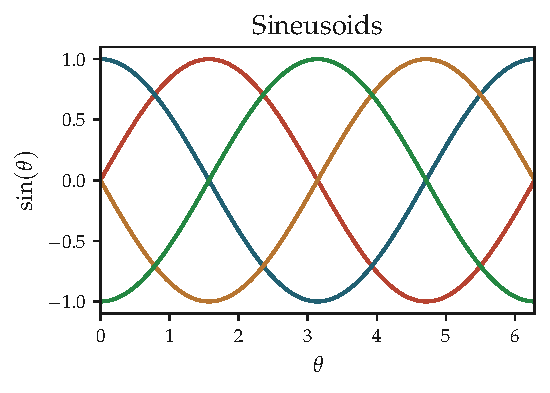
\includegraphics[width=0.75\textwidth]{example.pdf}
		\caption{An example plot with matching font scaling}
		\label{fig:example}
	\end{figure}
		
\end{document}